\documentclass[a4paper]{article}
\usepackage{geometry}
\usepackage{float}
\usepackage{longtable}
\usepackage{amsmath}
\usepackage[bottom]{footmisc}
\geometry{verbose,a4paper,tmargin=3cm,bmargin=2cm,lmargin=2cm,rmargin=3cm}
%\SweaveOpts{width=5.5, height=5.5}
\setlength{\parskip}{\medskipamount}
\setlength{\parindent}{0pt}
\usepackage{Sweave}
\begin{document}
\title{Surplus tests with MSE}
\author{Ernesto Jardim\footnote{ernesto.jardim@jrc.ec.europa.eu} (JRC)\\ Iago Mosqueira (JRC) \\ Colin Millar (JRC)\\ Chato Osio (JRC)\\ Aymen Charef (JRC)}
\maketitle
\begin{abstract}
ToDo
\end{abstract} 

\pagebreak
\section{Introduction}

The MSE runs on the ple4 dataset but it can be adapted to other datasets. The OM is conditioned using the stock assessment results and distinct S/R. The MP is based on the usual MSY HCR, with a $B_{trigger}$ and a $F_{target}$, and an additional harvest rate limit. All is dealt in relative terms. The stock status is estimated with a biomass dynamic model. The OEM introduces variability on the abundance index and bias both on the abundance index and catches. The IEM introduces bias on the catch. The bias on catch, both on the OEM and IEM must be linked so that catches on the OM are of the same level.


\begin{Schunk}
\begin{Sinput}
> sessionInfo()
\end{Sinput}
\begin{Soutput}
R version 2.15.0 (2012-03-30)
Platform: x86_64-pc-linux-gnu (64-bit)

locale:
 [1] LC_CTYPE=en_US.UTF-8       LC_NUMERIC=C              
 [3] LC_TIME=en_US.UTF-8        LC_COLLATE=en_US.UTF-8    
 [5] LC_MONETARY=en_US.UTF-8    LC_MESSAGES=en_US.UTF-8   
 [7] LC_PAPER=C                 LC_NAME=C                 
 [9] LC_ADDRESS=C               LC_TELEPHONE=C            
[11] LC_MEASUREMENT=en_US.UTF-8 LC_IDENTIFICATION=C       

attached base packages:
[1] splines   grid      stats     graphics  grDevices utils     datasets 
[8] methods   base     

other attached packages:
 [1] Hmisc_3.9-3      survival_2.36-14 xtable_1.7-0     plyr_1.7.1      
 [5] FLBioDym_0.1.2   FLAdvice_1.0     ggplotFL_0.1     ggplot2_0.9.1   
 [9] akima_0.5-7      FLash_2.5.0      FLCore_2.5.0     lattice_0.20-6  

loaded via a namespace (and not attached):
 [1] cluster_1.14.2     colorspace_1.1-1   dichromat_1.2-4    digest_0.5.2      
 [5] labeling_0.1       MASS_7.3-18        memoise_0.1        munsell_0.3       
 [9] proto_0.3-9.2      RColorBrewer_1.0-5 reshape2_1.2.1     scales_0.2.1      
[13] stats4_2.15.0      stringr_0.6        tools_2.15.0      
\end{Soutput}
\end{Schunk}

\pagebreak
\section{Methods}

\begin{itemize}
	\item Operating Model

	$N_{t+1,a+1}=N_{t,a}e^{-Z}$
	
	$R_{t+1}=f(S_{t})\rho$ where $\rho \sim LN(0,\sigma_{R}^2)$ and $f$:{segreg,b\&h,b\&h+AR1}

	$C_{t,a}=\frac{F_{t,a}}{Z_{t,a}}(1-e^{-Z})N_{t,a}$
	
	$Y_{t}=\sum_a C_{t,a}\bar{W}_{t,a}$
	
	\item Implementation Error Model
	
	$Y_{t}=\frac{TAC_{t}}{\beta_{t}}$ where $\beta \sim U(0.95\eta, 1.05\eta)$ 
	
	$\eta=a+b(TAC)$ if $TAC>min(C)$ or $TAC<max(C)$ 
	
	$\eta=1$ if $TAC>max(C)$ 

	$\eta=cthBias$ if $TAC<min(C)$ 

	\item Management Procedure
	
	$TAC_{t}=HCR(\hat{\Theta}_{t} | F_{trgt}, B_{trg}, HR_{max})$
	
	$\hat{\Theta}=g(\hat{C}_{t}, \hat{I}_{t})$ where $g$: biomass dynamic model 
	
	\item Observation Error Model
	
	$\hat{C}_{t}=C_{t} \alpha_{t}$ where $\alpha \sim U(0.95cthBias, 1.05cthBias)$
	
	$\hat{I}_{t} = B_{t} \gamma_{t}$ where $\gamma \sim LN(\lambda, \sigma_{I}^2)$ and $\lambda \sim U(0.95srvBias, 1.05srvBias)$	
		
\end{itemize}	

The scenarios simulated try to give insights about the doubts raised during the discussion of the factors that could have an impact on the estimation of MSY and indirectly on catch surplus.

\begin{itemize}
	\item Underestimation of catches - which is being modelled through the introduction of bias in catches provided to the assessment model by the OEM. It reflects the situation where company owners under-report catches to the coastal state. 
	\item Abundance index low quality - which is being modelled trough the introduction of bias and variability on the abundance index provided to the assessment model by the OEM. Bias models the effect of having surveys that don't cover the full distribution of the stock. A bias smaller than 1 reflects an underestimation of biomass and vice versa. It's common to use exploratory fishing surveys, which will most of the times look for hot spots of abundance and their estimates of abundance will most likely biased towards higher than reality abundances. On the other hand mixing surveys from different periods and carried out with several vessels, will increase the variability of the abundance index. 
	\item Lag between assessments - is modelled trough the introduction of years without assessment during which the TAC is kept constant as computed on the last assessment. More sophisticated approaches could be implemented if time allows. The simulation assumes that lags between assessments are regular, which is not (always ?) the case. It shouldn't be difficult to implement irregular assessment periods, that will reflect a lack of strategy towards management advice.
	\item Over-catch - it's implemented with two distinct Implementation Error Models (IEM), a constant ratio and a ratio that decreases linearly with the increase in TAC. The idea is that over-catch increases with the decrease in the TAC, which seems more realistic that keeping over-catch with a constant ratio.  
\end{itemize}     

\begin{table}[h]
\caption{Simulation scenarios}
% latex.default(scn, longtable = TRUE, file = "", first.hline.double = FALSE) 
%

\setlongtables


\begin{longtable}{lrrrrrr}
\hline
\multicolumn{1}{l}{scn}&\multicolumn{1}{c}{Btrig}&\multicolumn{1}{c}{CV}&\multicolumn{1}{c}{Ftar}&\multicolumn{1}{c}{aLag}&\multicolumn{1}{c}{srvBias}&\multicolumn{1}{c}{cthBias}\tabularnewline
\hline
\endhead
\hline
\endfoot
1&$0.5$&$0.2$&$1$&$1$&$1.0$&$1.0$\tabularnewline
2&$0.5$&$0.2$&$1$&$3$&$1.0$&$1.0$\tabularnewline
3&$0.5$&$0.2$&$1$&$5$&$1.0$&$1.0$\tabularnewline
4&$0.5$&$0.2$&$1$&$1$&$0.5$&$1.0$\tabularnewline
5&$0.5$&$0.2$&$1$&$3$&$0.5$&$1.0$\tabularnewline
6&$0.5$&$0.2$&$1$&$5$&$0.5$&$1.0$\tabularnewline
7&$0.5$&$0.2$&$1$&$1$&$1.0$&$0.5$\tabularnewline
8&$0.5$&$0.2$&$1$&$3$&$1.0$&$0.5$\tabularnewline
9&$0.5$&$0.2$&$1$&$5$&$1.0$&$0.5$\tabularnewline
10&$0.5$&$0.2$&$1$&$1$&$0.5$&$0.5$\tabularnewline
11&$0.5$&$0.2$&$1$&$3$&$0.5$&$0.5$\tabularnewline
12&$0.5$&$0.2$&$1$&$5$&$0.5$&$0.5$\tabularnewline
\hline
\end{longtable}\end{table}

\section{Results}

\begin{figure}[H]
\centering
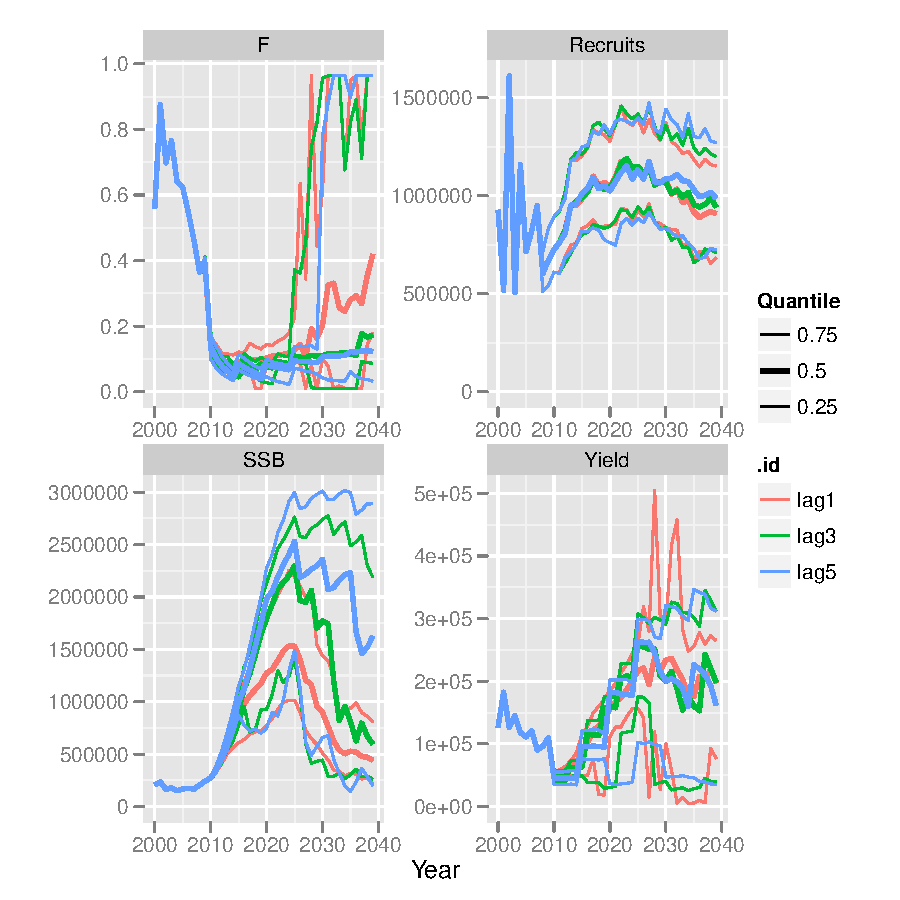
\includegraphics{MSE-004}
\caption{Projections with assessment lags of 1,3 and 5 years}
\label{fig:lags}
\end{figure}
 
\begin{figure}[H]
\centering
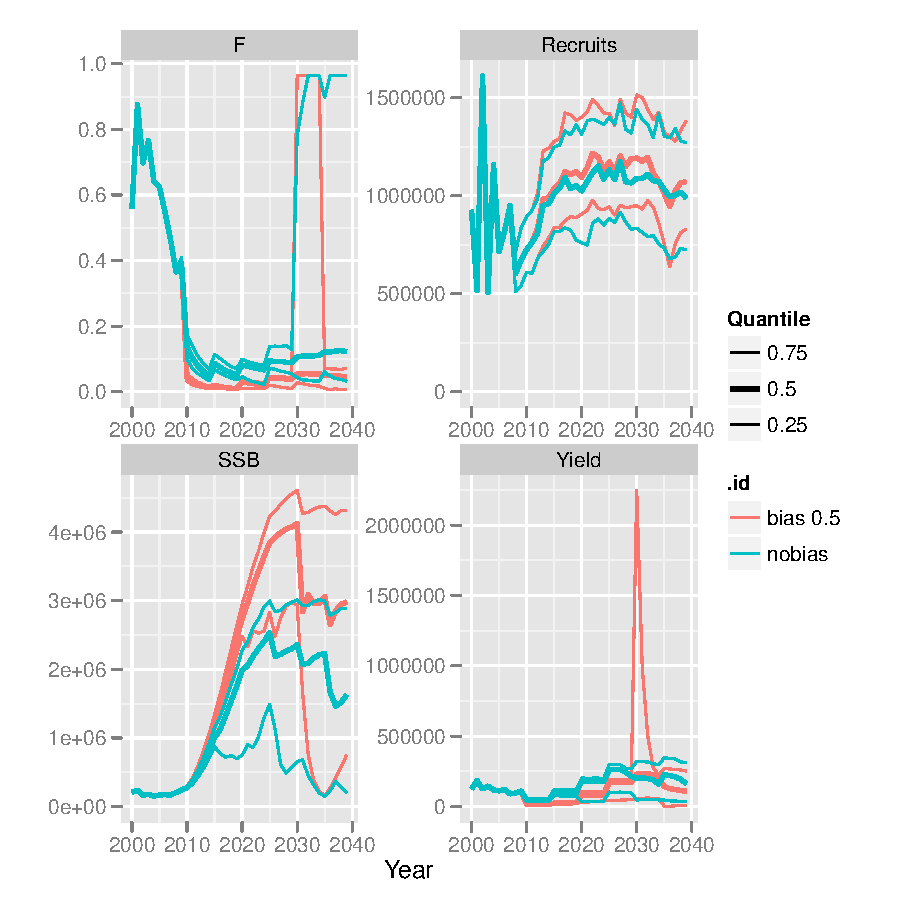
\includegraphics{MSE-005}
\caption{Projections with bias on the index of abundance}
\label{fig:srvBias}
\end{figure}

\begin{figure}[H]
\centering
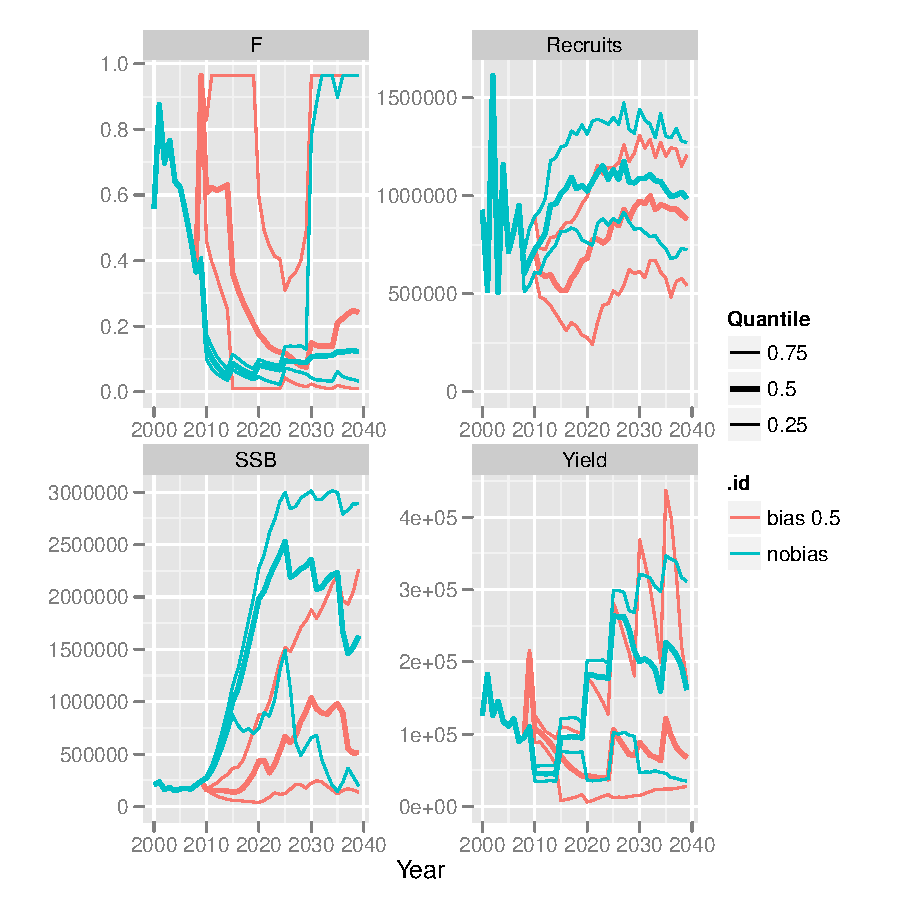
\includegraphics{MSE-006}
\caption{Projections with bias on catches}
\label{fig:cthBias}
\end{figure}

\begin{figure}[H]
\centering
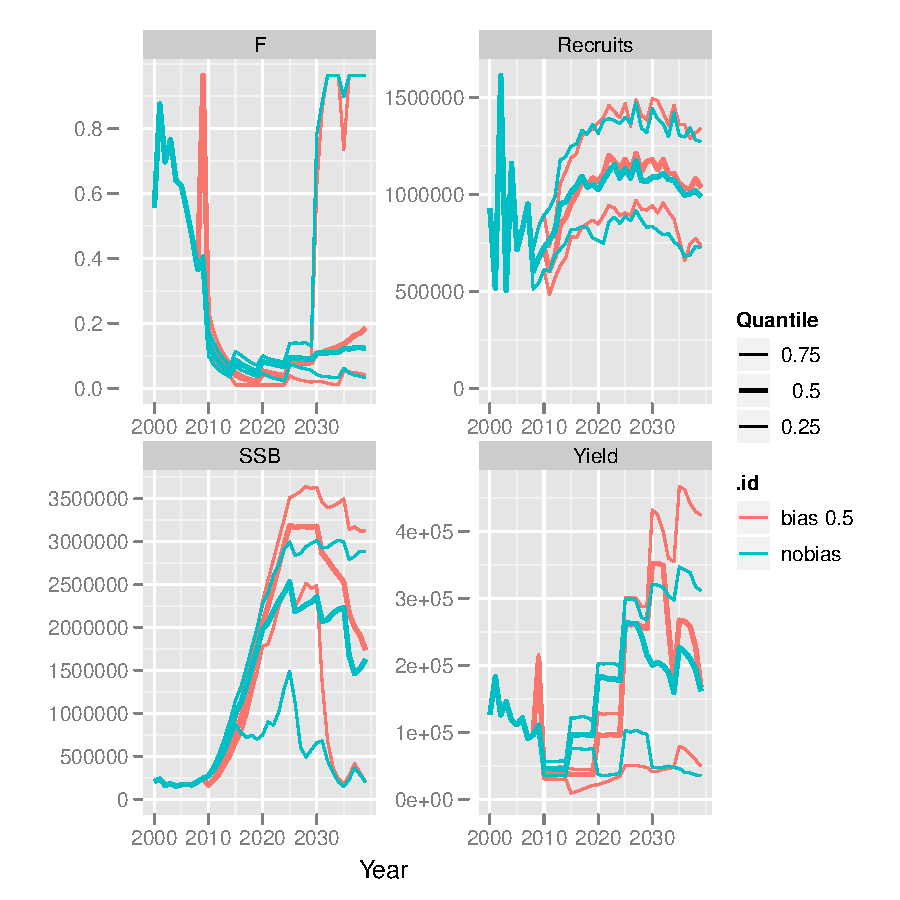
\includegraphics{MSE-007}
\caption{Projections with bias on catches and index}
\label{fig:2Bias}
\end{figure}

\section{Discussion}

This simulation study considers a TAC management system. It's not clear what would happen in a effort management system. Most likely the IEM could be implemented through limitations in effort or changes in catchability. However, considering DGMARE's comments on the enforcement of logbooks and future e-logbooks, there is the expectation that catches can be controlled.

\end{document}

